\documentclass[__main__.tex]{subfiles}

\begin{document}

\qtitle{С}{13}
Проводники в электростатическом поле. Теорема Ирншоу. Поле вблизи поверхности проводника. Ёмкость уединённого проводника. Конденсатор.\\

\begin{theorem}[Теорема Ирншоу]
    Всякая равновесная конфигурация покоящихся точечных электрических зарядов неустойчива, если на них, кроме кулоновских сил притяжения и отталкивания, никакие другие силы не действуют.
    \llabel{s13:irn}
\end{theorem}
\begin{minipage}{.65\linewidth}
    \begin{proof}
        Допустим, что какая-то система неподвижных точечных зарядов находится в устойчивом равновесии. Рассмотрим произвольный заряд $q$ этой системы, находящийся в равновесном положении. Не теряя общности положим $q>0$. Если $q$ сместится в бесконечно близкую точку $A'$, то ввиду устойчивости равновесия должна возникнуть сила, направленная к т. $A$ и стремящаяся вернуть $q$ в ту же точку. Пусть $\vec{E}$ -- электрическое поле, создаваемое всеми зарядами, кроме $q$, в точке $A'$ оно должно быть направлено к $A$. Окружим заряд замкнутой поверхностью $S$ такой, что остальные заряды расположены вне ее. На $S$ поле $\vec{E}$ направлено к т. $A$, следовательно, поток $\vec{E}$ через $S$: $\Phi_{S}(\vec{E)}$ отрицателен, но это противоречит теореме Гаусса: она требует, чтобы $\Phi_{S}(\vec{E})=0$, т.к. поток создается зарядам, расположенными все $S$. Получим противоречие.
    \end{proof}
\end{minipage}
\hfill
\begin{minipage}{.25\linewidth}
    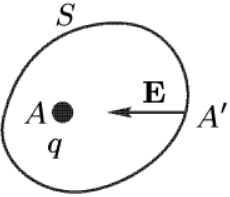
\includegraphics[width=1\linewidth]{С-13_1}
\end{minipage}\\

Рассмотрим проводник $V$ во внешнем электрическом поле. Если бы внутри него существовало электрическое поле $\vec{E}$, тогда свободные электроны в проводнике пришли бы в движение и равновесие электричества было бы невозможно. Для равновесия необходимо, чтобы $\forall\vec{r}\in{V}\vec{E}=\vec{0}$. Но тогда из уравнения Максвелла:
\begin{gather}
    \nabla\vec{E}=4\pi\rho,
\end{gather}
следует, что $\forall\vec{r}\in{V}\rho=0$ -- объемная плотность тока в проводнике равна нулю. Тогда, согласно Теор. \lref{s13:irn} \emph{все заряды расположены на поверхности проводника $S$}. Положим, что внутри проводника возникли заряды: притяжение одноименных зарядов приведет к их нейтрализации, а отталкивание разноименных -- к тому, что они разойдутся на максимальное расстояние и расположатся на поверхности тела. Из тех же соображений \emph{поверхностная плотность зарядов максимальна на участках проводника, обладающих максимальной кривизной}.
Тогда \emph{напряженность поля вблизи поверхности проводника} выражается как:
\begin{gather}
    \vec{E}=4\pi\sigma\vec{n},
\end{gather}
где $\sigma$ -- поверхностная плотность заряда, $\vec{n}$ -- внешняя нормаль к поверхности проводника $S$.

\begin{definition}
    Емкостью уединенного проводника с зарядом $q$ называют величину:
    \begin{gather}
        C=\frac{q}{\varphi},
    \end{gather}
    где $\varphi$ -- потенциал, создаваемого этим проводником электрического поля.
\end{definition}
$C$ зависит только от размеров и формы проводника, а также от окружающего его диэлектрика.

\begin{definition}
    Конденсатор -- физическое устройство, способное накапливать и сохранять электрический заряд и энергию электрического поля.
\end{definition}
Простейшая конструкция конденсатора -- два заряженных проводника с равными по модулю, но разными по знаку, зарядами, разделенные диэлектриком. Основная характеристика конденсатора -- его емкость $C$:
\begin{gather}
    C=\frac{q}{\varphi_1-\varphi_2},
\end{gather}
где $q$ -- заряд одного проводника (\emph{одной обкладки}), $\varphi_1$, $\varphi_2$ -- потенциалы обкладок.

\end{document}